\section{实验设计}
\subsection{ALU}\label{sub:alu}
\subsubsection{功能描述}
该 ALU 实现加法、减法、按位与、按位或、取反及无符号小于判断等基础运算功能,支持 8 位
与 32 位输入,输出 32 位结果,并在数码管上进行显示。
\subsubsection{接口定义}
\begin{table}[htp]
\caption{接口定义}\label{tab:signaldef}
\begin{center}
	\begin{tabular}{|l|l|l|p{6cm}|}
	\hline
	\textbf{信号名} & \textbf{方向} & \textbf{位宽} & \textbf{功能描述}\\ \hline \hline
	num1	&Input	&8-bit	&操作数1\\
	num2	&Input	&32-bits	& 操作数2\\
	op	&Output	&3-bits	& 操作码\\
	result	&Output	&32-bits & 计算结果\\
	\hline
	\end{tabular}
\end{center}
\end{table}

\subsubsection{逻辑控制}
本 ALU 模块采用组合逻辑控制方式,不使用时序触发的有限状态机(FSM)。由于 ALU 
运算为即时反应型逻辑(无时序依赖),其控制流程可简化为单周期组合逻辑响应,无需状态跳转。
模块通过将 8 位输入零扩展为 32 位,并根据 3 位操作码执行加、减、与、或、取反和小于判断等运算,非法操作码输出全 x。
ALU的控制逻辑使用组合逻辑电路实现,具体如下:
\begin{figure}[htbp]
    \centering
    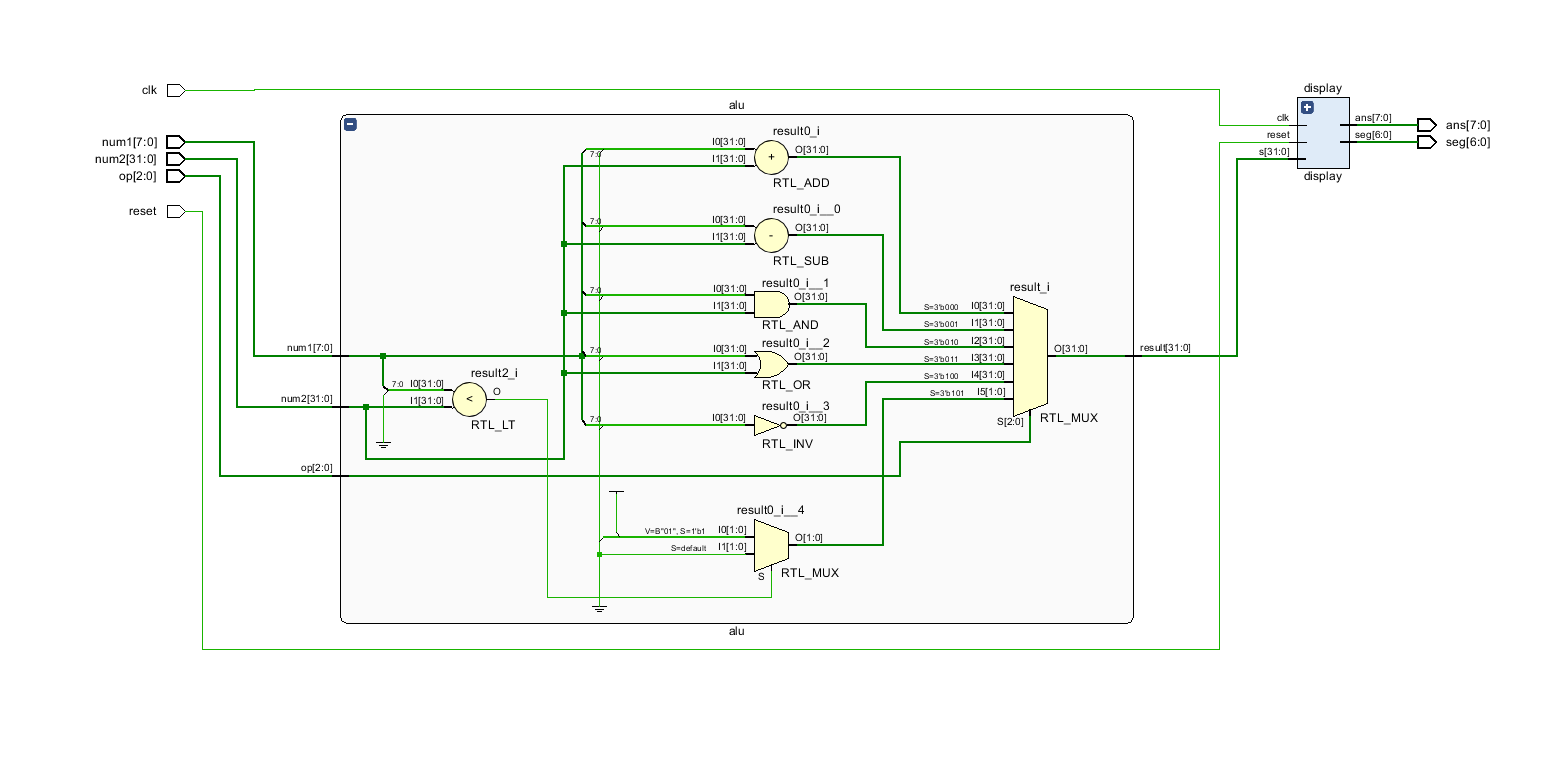
\includegraphics[width=0.7\textwidth]{image/yingjian.png}
    \caption{ALU控制逻辑电路}
	\label{fig:alu_control}
\end{figure}
\subsection{有阻塞4级8bit全加器}\label{sub:ctl}
\subsubsection{功能描述}
\subsubsection{接口定义}
\subsubsection{逻辑控制}
